\section{Week structure}
In the following sections we will go through the work done each week and who did the work on each of the individual task.
\subsection{Week one - Initialization and project development}
The first week was spent creating the basics of our project. In this week, our goal was to establish the foundation on which we would create the final scene and the interactive objects used in the calculations. 
On the graphical side of the project, we created a basic scene with two sphere objects to symbolise the final planets of our project. The methods for loading the sphere and very basic lighting of the scene was also implemented.
During this week, we also established the basic classes for handling the physics calculations. These would control the calculations regarding gravitational pull of every object towards each other and thereby bestow an acceleration upon the objects, which would in due time become the actual motion of the objects.
Most of the work done during this week was preparation. We set up a Git structure to account for the project, and established the fundamental data structure we were aiming to use. This structure was conceived to be a simulation object ("SimObjecT") containing two sub-objects - a graphical ("GraphicsObject") and a physical ("PhysicsObject") representation of the super-object - in separate classes, linked through a common position value kept in the SimObject, see figure \ref{GraphicsObjects}.
\begin{figure}[h]
\centering
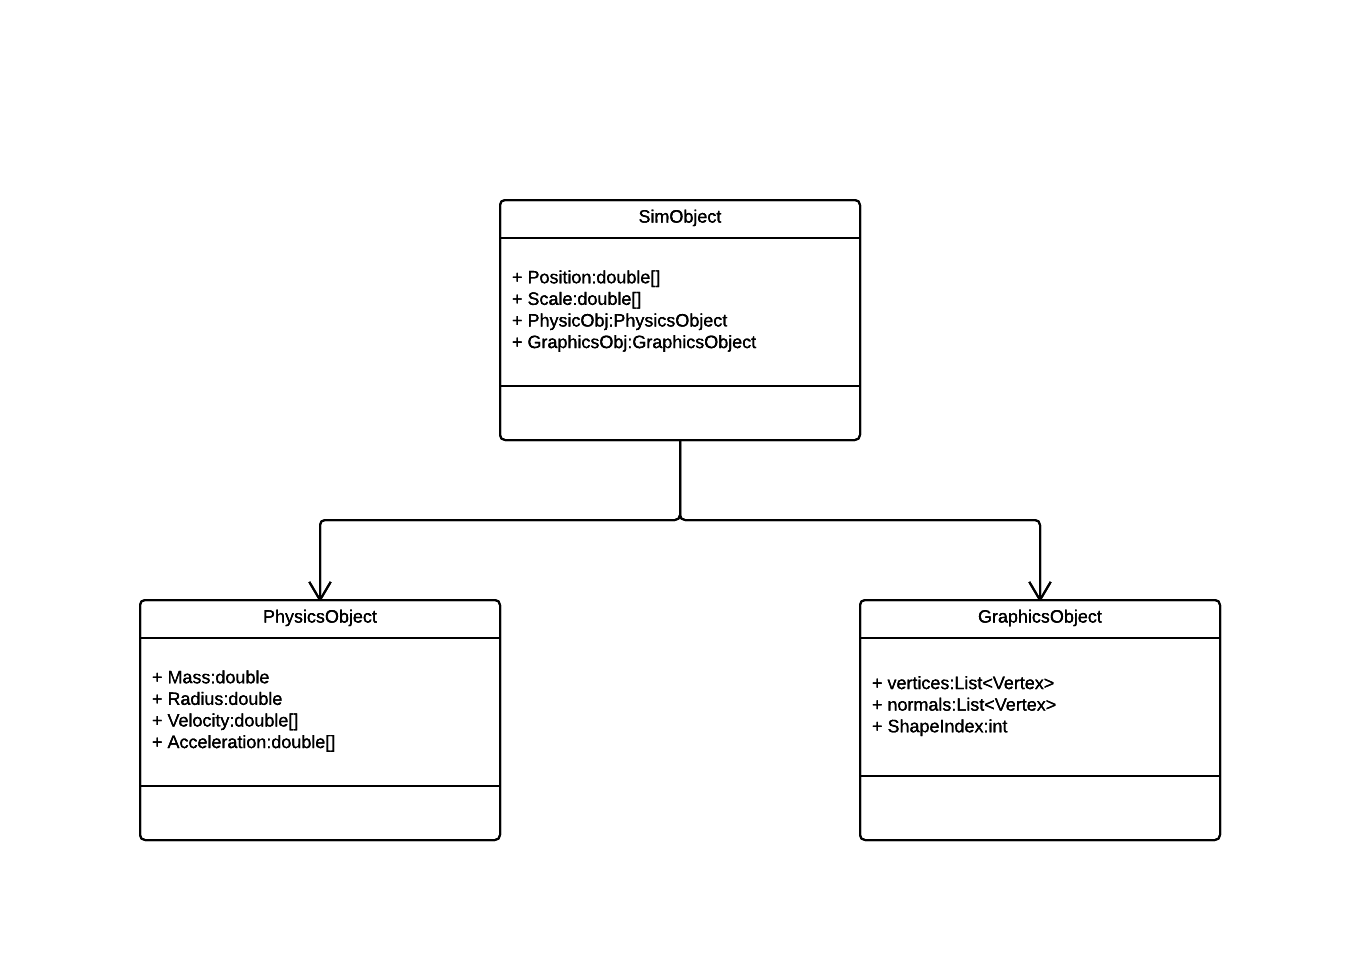
\includegraphics[scale=0.7]{GraphicsProjectObjects.png}
\label{GraphicsObjects}
\caption{Structure of the simulation objects and their physics and graphic objects}
\end{figure}
\subsection{Week two - Integration and transformation}
This week we integrated the different parts of the project for a unified physics and graphical simulation. There was some problems with graphical and physical integration, were the positions were not updated. 
Even after the integration were completed. There were some problems with moving the camera so that we could follow the moving planets. 
The physics were updated to produce transformation matrices which should move the objects around in the simulation. These change the current position of the graphical object. They needed to be moved through translation of their vertices which required a translation matrix.
\subsection{Week three}
Implementation of comet initialisation
Shading algorithm.

\subsection{Week Four}
Polishing of project and preparation for presentation
\textsl{}